%Copyright 2014 Jean-Philippe Eisenbarth
%This program is free software: you can 
%redistribute it and/or modify it under the terms of the GNU General Public 
%License as published by the Free Software Foundation, either version 3 of the 
%License, or (at your option) any later version.
%This program is distributed in the hope that it will be useful,but WITHOUT ANY 
%WARRANTY; without even the implied warranty of MERCHANTABILITY or FITNESS FOR A 
%PARTICULAR PURPOSE. See the GNU General Public License for more details.
%You should have received a copy of the GNU General Public License along with 
%this program.  If not, see <http://www.gnu.org/licenses/>.

%Based on the code of Yiannis Lazarides
%http://tex.stackexchange.com/questions/42602/software-requirements-specification-with-latex
%http://tex.stackexchange.com/users/963/yiannis-lazarides
%Also based on the template of Karl E. Wiegers
%http://www.se.rit.edu/~emad/teaching/slides/srs_template_sep14.pdf
%http://karlwiegers.com
\documentclass{scrreprt}
\usepackage{listings}
\usepackage{underscore}
\usepackage[bookmarks=true]{hyperref}
\usepackage[utf8]{inputenc}
\usepackage[english]{babel}
\usepackage{graphicx, wrapfig, subcaption, setspace, booktabs}
\usepackage{caption}
\usepackage{array}
\usepackage{longtable}
\captionsetup[figure]{labelformat=empty}
\hypersetup{
    bookmarks=false,    % show bookmarks bar?
    pdftitle={Software Requirement Specification},    % title
    pdfauthor={Jean-Philippe Eisenbarth},                     % author
    pdfsubject={TeX and LaTeX},                        % subject of the document
    pdfkeywords={TeX, LaTeX, graphics, images}, % list of keywords
    colorlinks=true,       % false: boxed links; true: colored links
    linkcolor=blue,       % color of internal links
    citecolor=black,       % color of links to bibliography
    filecolor=black,        % color of file links
    urlcolor=purple,        % color of external links
    linktoc=page            % only page is linked
}%
\def\myversion{1.0 }
\date{}
%\title
\usepackage{hyperref}
\newcolumntype{P}[1]{>{\centering\arraybackslash}p{#1}}
\newcolumntype{M}[1]{>{\centering\arraybackslash}m{#1}}
\begin{document}

\begin{flushright}
    \rule{16cm}{5pt}\vskip1cm
    \begin{bfseries}
        \Huge{SOFTWARE REQUIREMENTS\\ SPECIFICATION}\\
        \vspace{1.9cm}
        for\\
        \vspace{1.9cm}
        Simulated Computing System\\
        \vspace{1.9cm}
        \LARGE{Version \myversion}\\
        \vspace{1.9cm}
        Prepared by António Pedro Fraga\\
        \vspace{1.9cm}
        Cranfield University\\
        \vspace{1.9cm}
        \today\\
    \end{bfseries}
\end{flushright}

\tableofcontents

\chapter{Introduction}

\section{Purpose}
This document is a Software Requirements Specification of a project developed under under two modules, \textbf{Software Testing and Quality Assurance} and  \textbf{Requirements Analysis and System Design} at \textbf{Cranfield University}. It describes the implementation of a computing control system. This document is primarily intended to be proposed to the IT department for their approval and serve as a reference for the development of the system.


\section{Project Scope}

\par The software is a \textbf{simulator of a job control system}. It will be used by the IT department of Cranfield University so that it can explore different strategies to their current implementation. 
\par The developed software will include an \textbf{User Friendly Interface}, so that it can be used more easily. The simulation shall be capable of regulate its \textbf{inputs} so that it can compute a set of outputs.
\par The resulting application shall be a \textbf{reliable} and \textbf{efficient}, \textbf{cross-platform} program.

\section{Standards}

\subsection{Documentation}

\par This document follows the \textbf{Requirements Specifications template (IEEE Std 830-1998)}, selecting the most relevant topics for its scope. The \textbf{Test Plan} document shall follow the \textbf{IEEE 829 format}.

\subsubsection{Technical Documentation}

\par Good technical documentation is a key to the project scalability, helping future developers to have a better understanding of the whole project structure.
\par The project shall contain, at least, a \textbf{README} file created in its \textbf{GitHub} page. This file must include some topics:

\begin{itemize}
\item Tests status
\item Line coverage information
\item Project name
\item Description
\item Technologies
\item Informations about the development environment set up
\item Structure information (ex: location of important files)
\end{itemize}

\par The software shall also include documentation about the developed methods and its structure. All methods shall contain at least:

\begin{itemize}
\item Method name
\item Description
\item Arguments (type \& small description)
\item Return (type \& small description)
\end{itemize}

\subsection{Version Control}

This project shall have a \textbf{version control} system based on \textbf{GitHub}. The repository shall contain \textbf{two} main branches:

\begin{itemize}
\item Deployment - Containing a product release history
\item Development - Containing a merge of the newly developed features
\end{itemize}

\par A branch shall be created every time a new feature starts its development.
\par The \textbf{feature} branch shall be merged with the \textbf{Development} branch every time its development has came to an end.
\par The \textbf{Development} branch shall be merged with the \textbf{Deployment} branch every time a new version of the product is released.

\subsection{Requirements}

A requirement should be written using a specific format, containing a tuple of of three expressions:

\begin{itemize}
\item Actor
\item Action
\item Reason
\end{itemize}

\par Thus, the template should be: As an \textbf{$<$actor$>$}, I want to \textbf{$<$action$>$}, so that \textbf{$<$reason$>$}.
\par Every requirement should be split in sub requirements every time the development effort is high.



\subsection{Naming}
A naming convention is a set of rules for selecting the character sequence to the identifiers of variables, classes, modules or implemented methods. There are different patterns that can be adopted when defining a convention:

\begin{itemize}
\item \textbf{PascalCase (UpperCamelCase)} - the first letter of each word composing the identifier is capitalized.
\item \textbf{Snake_case} - the elements of the compound words are separated with one underscore character and no spaces. The initial character of each element is lowercased, except for the first character, that can be both upper or lower case (‘snake_case’ or ‘Snake_
case’).
\end{itemize}

\subsubsection{Files}

\par C++ code shall be stored in \textbf{.cpp} files, whereas functions and variables definitions should be carried by \textbf{header} or \textbf{.h} files. File names shall follow the \textbf{snake_case} convention with the first character being uncapitalised.

\subsubsection{White spacing}

\par Blank lines improve readability by creating sections of code logically related. 
\par Every statement shall be correctly indented. The indentation increases by a \textbf{tab} if the previous line is:
\begin{itemize}
\item \textbf{\{} a left brace
\item \textbf{[} a left bracket
\item \textbf{(} a left parenthesis
\end{itemize}
The matching closing token must be the first in a line, restoring the previous indentation.
Blank spaces shall be used in some circumstances:

\begin{center}
    \begin{tabular}{|p{8cm}|p{6cm}|}
        \hline
	    Description & Example\\
        \hline
	    A keyword followed by the \textbf{left parenthesis} should be separated by a whitespace. \newline For example, there should be a space after an if or a while keyword. &  – while (true) \{ ... \newline – return (1 + 1); \newline – if (job.is_short()) \{ ... \\
	    \hline
	    The method \textbf{return type} shall be followed by a white space. & \textbf{double} get_usage_price() \\
	    \hline
	  	Every \textbf{comma} shall be followed by a line break or a white space. & insert_state(i\textbf{, }j\textbf{, }job); \\
	  	\hline
	  	Every \textbf{semicolon} at the end of a statement shall be followed with a line break. & i++\textbf{;}\newline j++\textbf{;}\\
	    \hline
	    Every \textbf{semicolon} in the control of a loop shall be followed by a white space. & for (int i = 0\textbf{; } i $<$ v.size()\textbf{; }i++) \{ ...\\
	    \hline
    \end{tabular}
\end{center}

\subsubsection{Classes}

\par Classes should be defined as names written in the \textbf{PascalCase} convention. Acronyms and abbreviations should be avoided, unless the abbreviation is widely used.

\subsubsection{Methods}

\par The name of each method shall start with a verb in the infinite form, being a \textbf{verb-name} pair. This name shall be written in \textbf{snake_case}. It should be self-explanatory and concise.

\par \textbf{Examples:} is_short(), is_medium, get_name(), get_price()

\subsubsection{Variables}

\par Variables shall be written in \textbf{snake_case}. The use of descriptive names is required, avoiding single characters names, except for loops. Abbreviations shall be avoided as well. All variables must be declared in the top of the method body, whit a blank line between this declaration and the rest of the method, forming an \textbf{instantiation block}. The names (\textbf{i}, \textbf{j}, \textbf{k}) are reserved for iteration purposes. 
\par Constant declarations must follow a \textbf{SNAKE_CASE} convention. The developer shall write them entirely with capital characters.


\subsubsection{Branches}

\par Branches shall be written in \textbf{snake_case}. Every branch shall have a name related with the developed feature. 

\chapter{Overall Description}

\section{Product Perspective}
\par The product is a stand-alone system. This system shall contain \textbf{at least} 128 nodes with \textbf{at least} 16 cores per node. It will be used by a set of simulated users that can be classified as:

\begin{itemize}
\item IT support
\item Researchers
\item Students
\end{itemize}

\par The IT support simulated users have an \textbf{infinite} budget, therefore is permitted to them to run as many jobs as they like. In other hand, the Students shall have a constant budget, which is a smaller amount compared to the Researchers budget. This budget confines the amount of jobs that a user is permitted to run. The system usage has a price per core, that shall be decreased from the simulated budget every second.
\par The users can use the system by submitting jobs. This jobs have a two main characteristics, the amount of time that will use the system (running time), and the amount of system cores it will use. Thus, there are four types of jobs:

\begin{itemize}
\item Short - can take up to 2 nodes for no more than 1 hour. 10\% of the machine is reserved for these kind of jobs.
\item Medium - can take up for 10\% of the total number of cores for no more than 8 hours. 30\% of the system is reserved for this queue.
\item Large - can take up for 50\% of the total number of cores for no more than 16 hours. 70\% of the system is reserved for this queue.
\item Huge - can only run from 1700 of Friday to 0900 of Monday, reserving the whole machine. During this time, no other job can be executed.
\end{itemize}

\par Every time a simulated user submits a job, a scheduler shall define whenever that job is going to run. This scheduler manages the amount of computational resources at every second.


\section{Product Functions}
An user of the simulation shall be able to regulate a set of the inputs:

\begin{itemize}
\item Number of jobs \footnotemark
\item Number of users \footnotemark[\value{footnote}]
\item Student Budget \footnotemark[\value{footnote}]
\item Researcher Budget \footnotemark[\value{footnote}]
\item Simulation date - the date when the first job submission is done.
\item Requests span - the time span that a job can be submitted in.
\item Number of nodes
\item Number of cores
\end{itemize}

The simulation shall produce a set of outputs regarding:

\begin{itemize}
\item The number of jobs processed in each queue (throughput) per week
\item The actual number of machine-hours consumed by user jobs
\item The resulting price paid by the users
\item The average wait time in each queue
\item The average turnaround time ratio, i.e. the time from placing the job request to completion of the job divided by the actual runtime of the job
\item The economic balance of the centre, calculated by subtracting from the actual price the operating costs
\end{itemize}

\footnotetext{The user shall decide whether this number is randomly defined following a linear distribution or is a constant value.}


\section{User Documentation}

\par The software shall have an \textbf{User Manual}, indicating which features can be explored. The manual should include a \textbf{screen-shot} of the \textbf{User Interface} along with an explanation of every possible action. The screen shot shall clearly indicate which \textbf{spin box} value is related to each input. The manual shall also include an explanation of the simulation output. Every output value shall be clarified, enlightening the user about its meaning.

\section{Assumptions and Dependencies}

\par For simplification purposes, it is assumed that the scheduler works on a basis of a \textbf{First Come, First Served} methodology. 
\par The running time of each job and the interval between job submissions follow \textbf{exponential distributions}.
\par The number of cores each job uses is generated following a linear distribution. The limits are defined according to each job type:
\begin{itemize}
\item Short: 1 core to 2 nodes of total cores
\item Medium: 2 nodes to 10\% of total cores
\item Large: 10\% nodes to 50\% of total cores
\item Huge: total number of cores
\end{itemize}
\par Every time an input is defined randomly, it follows a linear distribution.
\par It is assumed that only huge jobs can run during weekends, no other queue can be active during this period.
\par The default values of the \textbf{Operational Cost} and \textbf{Usage Price} shall be assumed as \textbf{£0.000475} and \textbf{£0.000014} respectively. The operational cost, is considered to have a constant value \textbf{per second}. The usage price is considered to have a constant value \textbf{per core second}. Further information about the calculations of these values can be found in the \textbf{appendixes} section.


\chapter{System Features}
This section defines the functional requirements of this system.
\begin{center}
    \begin{longtable}{|M{1.5cm}|M{4cm}|M{8cm}|}
        \hline
	    Identifier & Name & Description\\
        \hline
        SF01 & Number of Users & As a simulation user, I want to be able to regulate the number of simulated users, so that I can change the default configurations.  \\
        \hline
        SF02 & Number of Jobs & As a simulation user, I want to be able to regulate the number of simulated jobs, so that I can change the default configurations.  \\
        \hline
        SF03 & Student Budget & As a simulation user, I want to be able to regulate the Student Budget, so that I can change the default configurations.  \\
        \hline
        SF04 & Researcher Budget & As a simulation user, I want to be able to regulate the Researcher Budget, so that I can observe what kind of effects it will have on the simulation outputs.  \\
        \hline
        SF05 & Date & As a simulation user, I want to be able to define what is the start date of the simulation, so that I can explore every possible start date.  \\
        \hline
        SF06 & Requests Time Span & As a simulation user, I want to be able to define the value of the requests value span, so that I'm able to observe any output values fluctuations.  \\
        \hline
        SF07 & Number of nodes & As a simulation user, I want to be able to define the number of system nodes, so that I can observe what kind of effects it will have on the simulation outputs.   \\
        \hline
        SF08 & Cores per node & As a simulation user, I want to be able to define the number of system cores per nodes, so that I can observe what kind of effects it will have on the simulation outputs.   \\
        \hline
        SF09 & Run & As a simulation user, I want to be able to run the simulation, so that I can observe the simulation outputs.   \\
        \hline
    \end{longtable}
\end{center}


\chapter{Other Requirements}

\section{Performance}

Performance shall be an important quality metric int this system. A system with \textbf{n} jobs shall schedule their running times with a \textbf{time complexity} of \textbf{O(n log(n) + nk)}, k being the average distance between the job submission and a free slot to run the job. Regarding \textbf{memory}, the system shall have a \textbf{linear complexity}. Further explanations about this subject can be found in the appendixes section.

\section{Scalability}
The system shall be scalable. The chosen design shall permit future implementations. Code must be refactored every time a better design approach is found.

\section{Reliability}

The system must be 100\% reliable, which means that it must be able to function according to its specification under normal circumstances. The probability of failure should be null.

\section{Portability}

The resulting program shall be \textbf{cross-platform}, being able to execute on most of the operating systems and/or machines.

\chapter{Appendixes}

\section{Appendix A: Project Plan}

The project plan could be represented with a \textbf{Gantt Chart}. This chart is capable of representing dependencies between tasks, and each task duration.
\begin{figure}[!htb]
  \centering
  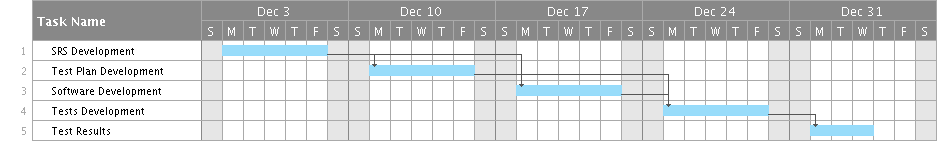
\includegraphics[width=\linewidth]{ProjectPlan.png}
\end{figure}

\section{Appendix B: Operational Cost \& Usage Price}

\par The default \textbf{usage price} is assumed to have the same value as \textbf{Archer}, the UK national supercomputing system. This system has a cost of \textbf{5p} per core hour. Thus, for each second:

\begin{center}
	$
		UP per core = 0.05 / 60
	$
\end{center}

\par The default \textbf{operational cost} is calculated with an average of costs that the centre has. 
\par Firstly it's assumed that the simulated system is a \textbf{green} supercomputer, therefore it has a power supply of \textbf{60KW}. In the United Kingdom, a KW costs \textbf{£0.0285 per hour}. Thereby, it's obtained a value of \textbf{£0.0285 per minute}, and $0.0285 / 60$ per second:
\begin{center}
	$
		Energy Cost = 0.0285 / 60
	$
\end{center}
The system is assumed to have a team of \textbf{10} elements making \textbf{£60.000} per year:
\begin{center}
	$
		Personel Cost = 60000 * 10 / 365 / 24 / 60 / 60
	$
\end{center}
The building maintenance costs an average of \textbf{£10.000} per year:
\begin{center}
	$
		Building Maintenance = 10000 / 365 / 24 / 60 / 60
	$
\end{center}
Every second, the default \textbf{operational cost} of the system is:
\begin{center}
	$
		Operational Cost = Energy Cost + Personel Cost + Building Maintenance
	$
\end{center}

Despite of having this default value, \textbf{the operational cost} can be changed as an input variable.

\section{Appendix C: Implementation}

\par Jobs will be generated randomly, having attributes characterized by the set of rules defined in this document. It is created an \textbf{array} of \textbf{Jobs}, sorted by \textbf{date of submission}. Every date will be stored as an \textbf{UNIX timestamp}, which is represented by the total number of seconds counted from \textbf{January 1st, 1970 at UTC}. This date is named as \textbf{UNIX Epoch}.

\begin{figure}[!htb]
  \centering
  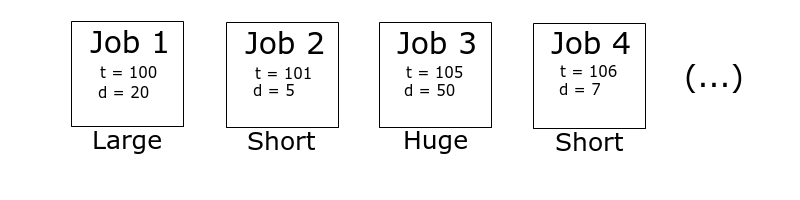
\includegraphics[width=\linewidth]{jobs.png}
\end{figure}

\par Jobs will be allocated to a random user. The \textbf{scheduler} will set a start time for each job on a basis of a \textbf{First Come, First Served} methodology. Since it will be important to keep track of the system state (queues computational resources available), it will be created a \textbf{vector} of \textbf{States}. 
\par This vector contains the available computational resources at each \textbf{start} and \textbf{end} time of a job. Therefore, every time a job is analysed, the scheduler algorithm will add \textbf{two states} to this vector. A state representing the available computational resources once the job starts, along with the occurrence time of the event \textbf{(start)}, and a different state representing the available resources once the job running life comes to an end, containing the timestamp of the occurrence as well.

\begin{figure}[!htb]
  \centering
  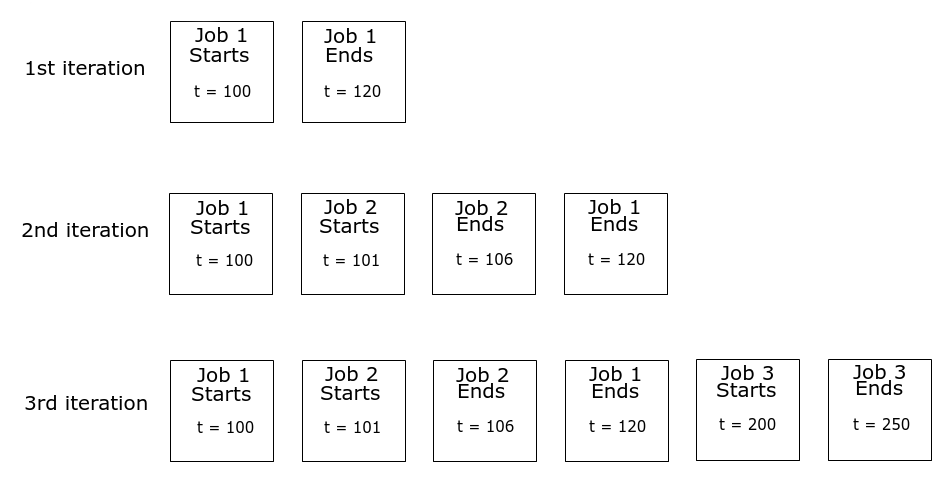
\includegraphics[width=\linewidth]{iterations.png}
\end{figure}

\par This vector shall be kept sorted every time two states are added to it. This way it will be easier to keep track of available \textbf{"running slots"}, which represent the nearest time the system is available to run a certain job.
\par Therefore, for purposes of performance, it can be saved the index to start looking for a free spot.
\par One knows that, as the \textbf{Job 2} is being scheduled, it is impossible to start it before the start date of \textbf{Job 1}. Since the array of Jobs is sorted by submission date, one can keep the \textbf{index} corresponding to future dates, or dates that will still be analysed by the algorithm. 
\par Thus, this procedure, achieves a time complexity of \textbf{O(n log(n) + nk)}. The initial \textbf{O(n log(n))}, is the weight of sorting the array of jobs, whereas the extra \textbf{nk} corresponds to the iterating process through the vector of jobs, and the vector of states. Note that when iterating through the states vector, only future states are analysed. This is a good improvement comparing to the quadratic algorithm of iterating through every state every time the next "free slot" to run a job is needed.
\par The memory complexity of this algorithm is \textbf{linear}, because only a vector of states and a vector of jobs are kept in memory, a long with some constant values like the \textbf{index} of future dates.

\section{Appendix D: Analysis Models}

\subsection{Use Cases Diagram}

\begin{figure}[!htb]
  \centering
  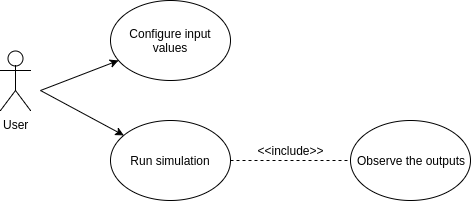
\includegraphics[width=12cm]{usecases.png}
\end{figure}

\subsection{Data Flow Diagram}

\begin{figure}[!htb]
  \centering
  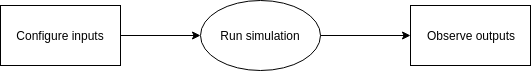
\includegraphics[width=12cm]{dataflow.png}
\end{figure}

\end{document}
